%%% -*-LaTeX-*-

\chapter{System Impact}
\label{chap:impact}

We saw how the Zero Copy promises savings of resources and enhanced performance 
in the previous chapters. To put things in the context of resource utilisation and
 to quantify performance gains, we profiled our benchmark code for memory bandwidth 
 and some other interesting metrics. One interesting observation from our initial 
 attempts was that our profiling code shouldn't interfere with the timing of our highly performant 
 benchmark which churns out millions of operations per second and microsecond latencies. 
 We searchaed for light weight profiling methods which adds minimal overheads.
 We ended up using Intel\textregistered's Performance Counter Monitoring module~\cite{intelpcm}. 
 An interesting thing about measuring performance 
 of a modern CPU is that almost all of the metrics of significance exist outside of the cores.
 The newer generation CPUs since the Sandy Bridge\textregistered microarchitecture provide an uncore performance 
 monitoring unit and we can use tools such as perf~\cite{perftool} to instrument these performance 
 counters. 

\section{Memory Bandwidth}
In a modern In-Memory Database server, DRAM utilisation is the most precious resource~\cite{ramcloudfast}. 
 Available memory bandwidth is also at a premium since there is a direct correlation between Memory Bandwidth
 utilisation and DRAM latencies and starvation. Since uncore events will give the most accurate measurements,
 we explored all uncore events that induce pressure on the memory controller. We found that 
\texttt{LLC\_MISSES X 64} (cache line size) is an interesting metric, but there was a problem that it wouldn't account for prefetch 
 misses. We went for the more accurate \texttt{MEMORY\_BW\_READS} and \texttt{MEMORY\_BW\_WRITES} metrics which are derived from 
 \texttt{CAS\_COUNT.RD} and \texttt{CAS\_COUNT.WR} metrics which are the number of cache lines read and written in the sampling 
 interval. We used an interactive reporting tool written on top of perf with named mappings for these events
 to measure this metric.


\begin{figure}[t]
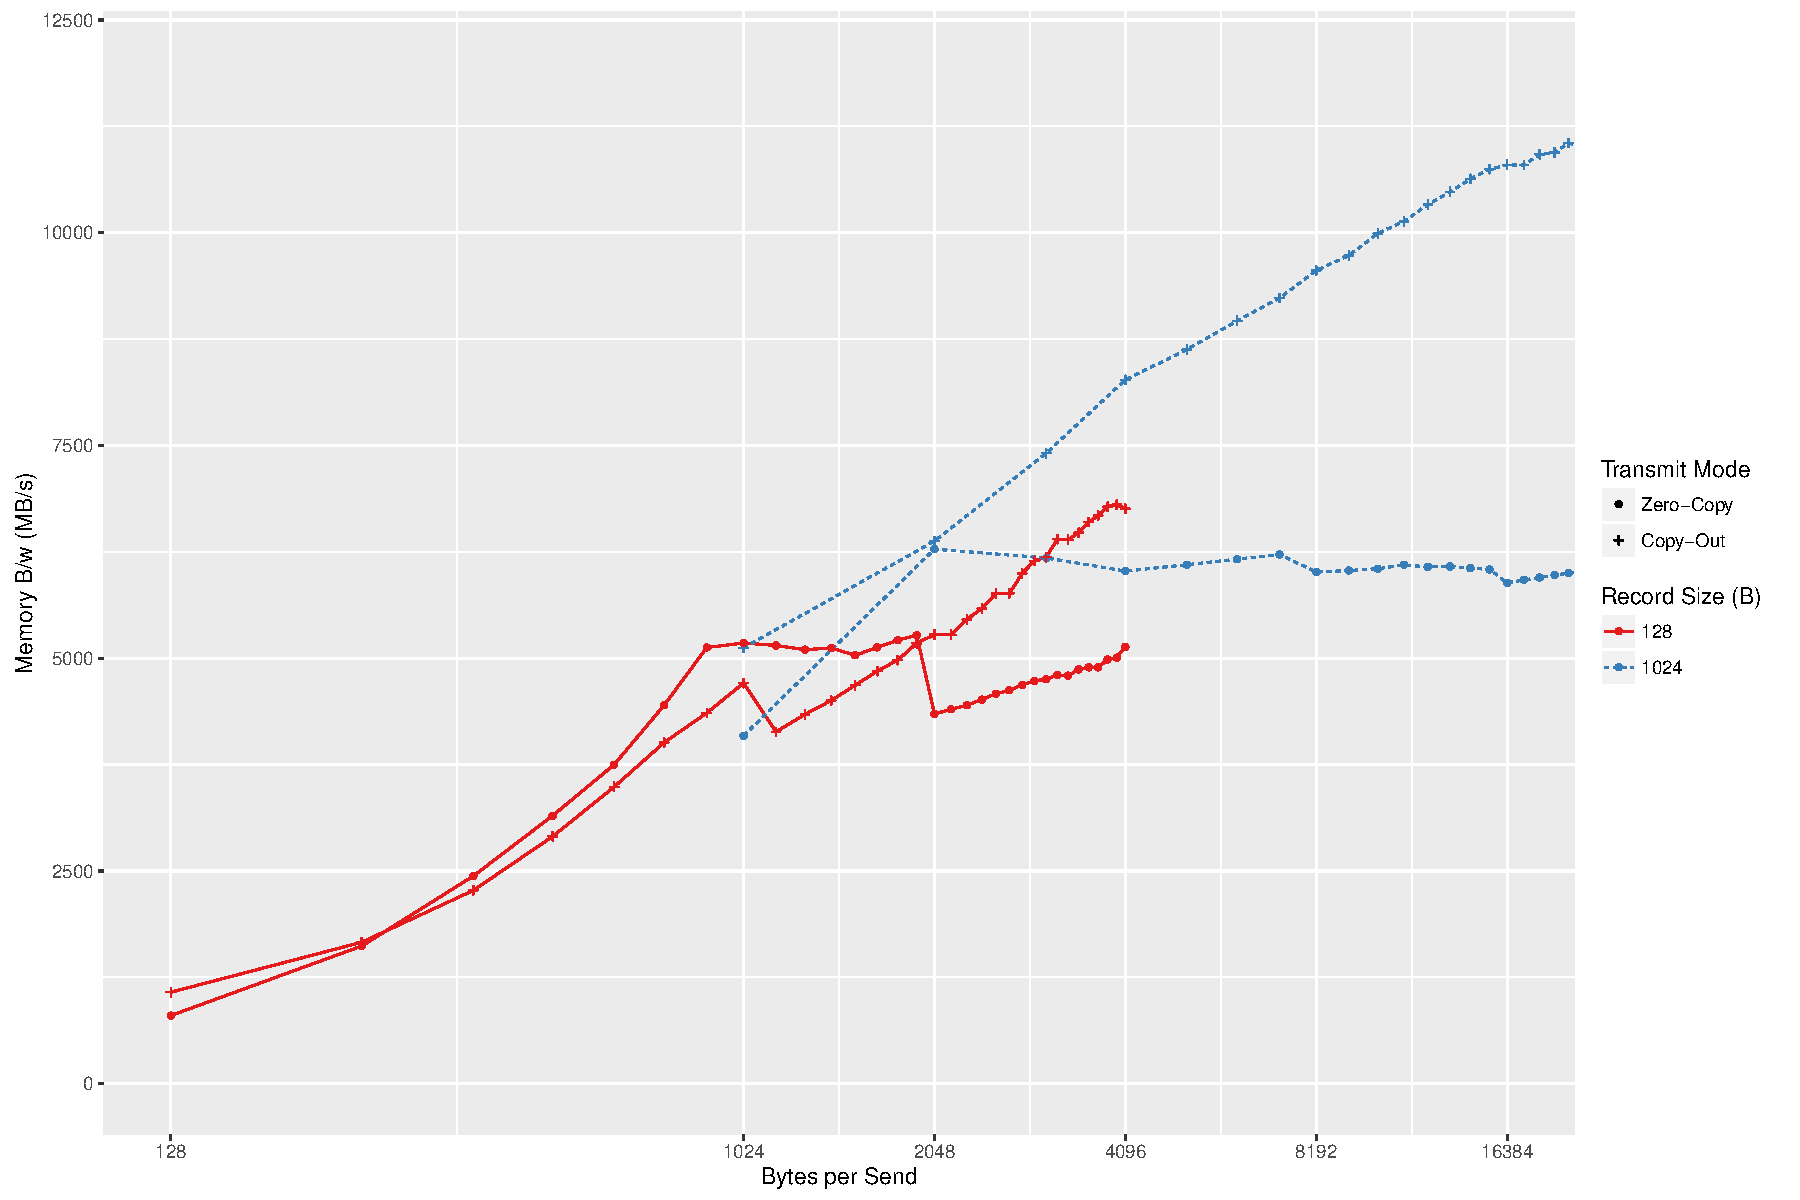
\includegraphics[width=\textwidth]{fig-membw.pdf}
\caption{Measured memory bandwidth impact on the system during transmission.}
\label{fig:membw}
\end{figure}

\begin{figure}[H]
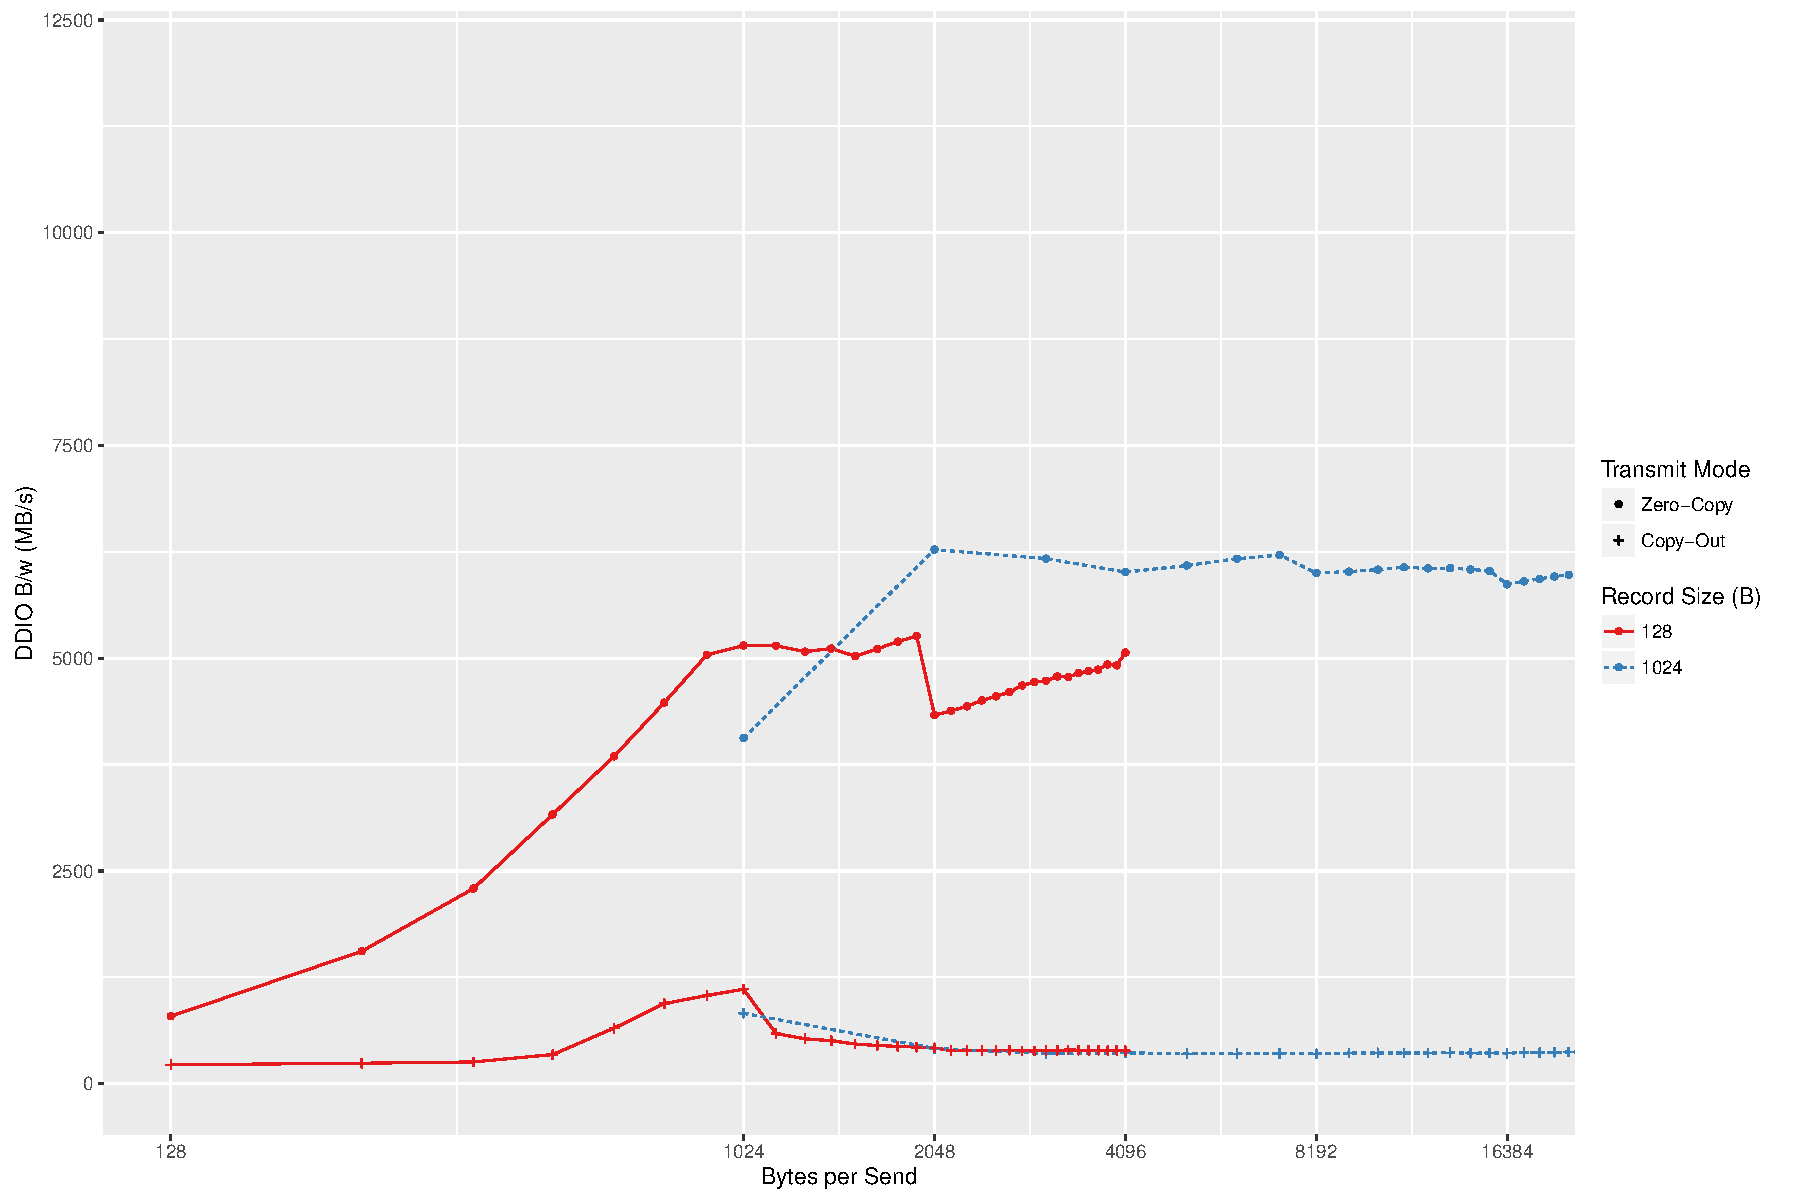
\includegraphics[width=\textwidth]{fig-ddiobw.pdf}
\caption{DRAM accesses (MB/s) LLC misses from DDIO vs Throughput}
\label{fig:ddiobw}
\end{figure}

\begin{figure}[t]
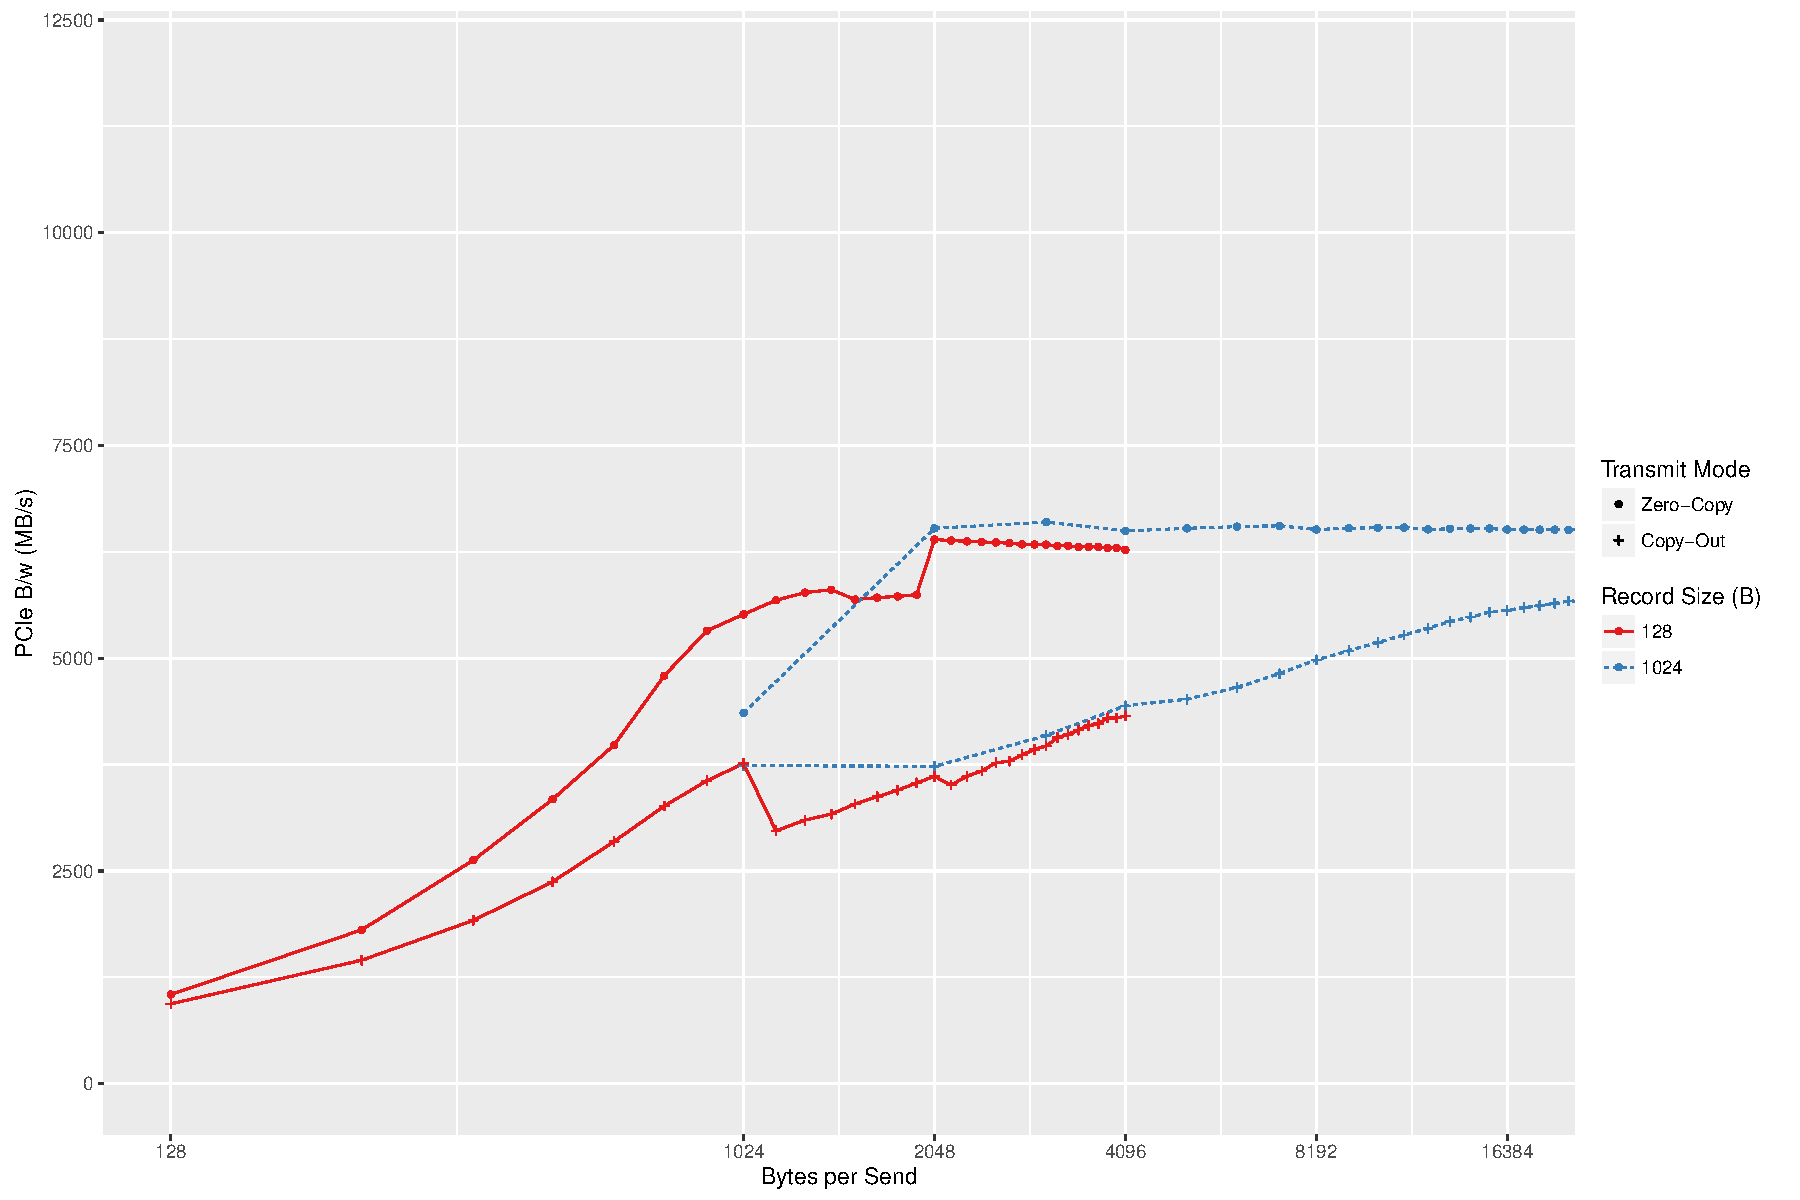
\includegraphics[width=\textwidth]{fig-pciebw.pdf}
\caption{DRAM accesses (MB/s) due to LLC misses due to PCIe}
\label{fig:pciebw}
\end{figure}

